\chapter{Effect of horizontal resolution on simulated larval retention patterns}\label{Chap2}

\clearpage
\section{Introduction}\label{Chap2Intro}

Interest in the early life stages of marine organisms has increased \citep{Stra1993,Haven1995,Levi2006,GawaMoni2007,CoweSpon2009} in particular for understanding larval transport and dispersal patterns \citep{Youn1995,GreeMayp2015,Leis2021} due to their key role in the ecology of marine organisms \citep{MoseSmit1993} and potential usefulness in decision making for the management of \acrfull{mpa} \citep{DaloBogd2015}. Many marine species have pelagic early life stages in their life cycle \citep{Haven1995}, being this phase of locomotion essentially driven by ocean currents and species-specific behaviours \citep{Levi1990,CowePari2006,DaloBogd2015}.\\

In the case of sessile organisms, such as scallops and corals, concepts such as larval transport, larval dispersal and population connectivity have been formally defined \citep{PineHare2007}. Fig. \ref{Chap2LarvalTransport}, shows \textbf{larval transport} as the horizontal translocation of a larva between points $X_{1}Y_{1}$, and $X_{2}Y_{2}$, where $X$ and $Y$ are the horizontal axes, perpendicular and parallel to the coastline respectively (to simplify, this definition ignores the vertical axis $Z$). On the other hand, \textbf{larval dispersal} refers to the spread of larvae from a spawning source to a settlement site (a geographic point from which the adult will have limited or no mobility). We note that larval transport is a component of larval dispersal. Finally, \textbf{population connectivity} is the exchange of individuals among geographically separated subpopulations. We note that larval dispersal is a component of population connectivity, and therefore larval transport too. In the case of pelagic or demersal organisms such as fish, these general concepts also apply but the movement of adults is also an important component of population connectivity.\\

During larval transport, organisms are dragged by currents and depend on environmental conditions to survive, whether temperature and/or food \citep{NocrShaw1984}, and currents may allow larvae to match their food source location \citep{CuryRoy1989}. It is in this context that larval drift models, which allow tracking the trajectory of eggs and larvae through a virtual environment, are a fundamental tool for understanding the transport patterns of different species. However, before interpret modelling results it is recommended to perform a sensitivity analysis to test the robustness of these results \citep{PeckHufn2012,SimoSieg2013}. Sensitivity analysis examines how a model's behaviour is affected by changes in its parameters and it can also refer to how the response variable changes when a model parameter is modified \citep{Hamb1994,Inga2008}.\\

In larval drift models, results may be sensitive to the number of released particles \citep{SimoSieg2013}, to lethal temperature \citep{BrocLett2008}, to wind frequency forcing \citep{FlorTam2019}, to the spatial resolution of the forcing currents \citep{GaraKapl2014}, etc. Since particle number has already been thoroughly studied and we have determined a robust number in previous experiments (not shown here), and lethal temperature and wind frequency have already been tested in the marine ecosystem off Peru, our focus will be on exploring whether spatial resolution significantly affects the overall patterns of larval transport and retention at the continental shelf scale.\\

\begin{figure}[H]
	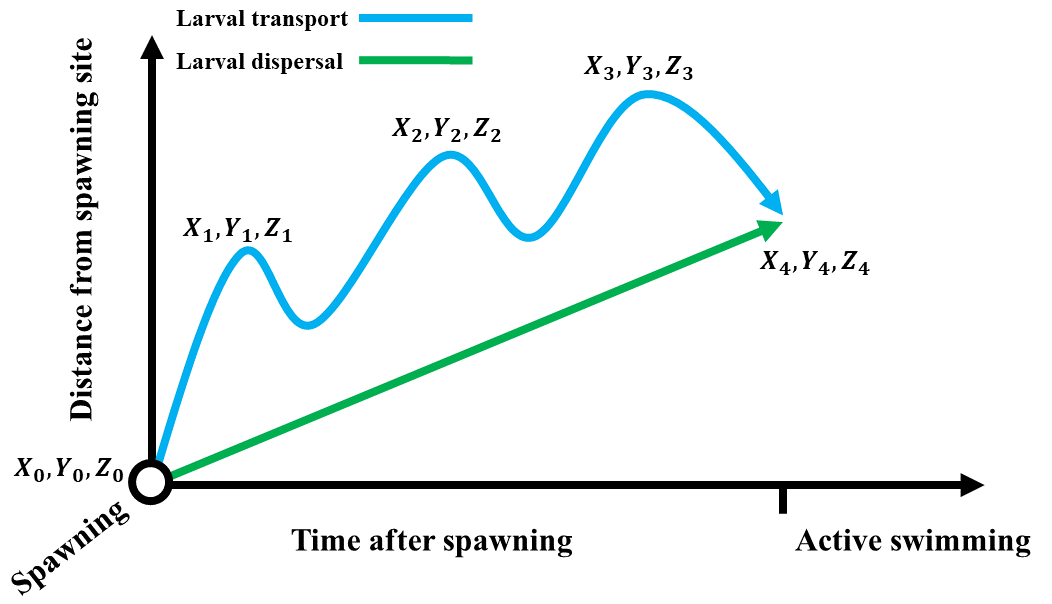
\includegraphics[width=1.0\textwidth]{figures/Chap2LarvalTransport.png}
	\centering
	\caption{Schematic representation of larval transport and larval dispersal processes. Note that the sum of the larval transport distance is greater than the dispersal distance. All locations ($X_{n},Y_{n},Z_{n}$) are pelagic.}
	\label{Chap2LarvalTransport}
\end{figure}

\clearpage
\section{Methods}\label{Chap2Meth}

An \acrfull{ibm} simulates populations and communities by following individuals and their properties \citep{DeanGrim2014}. As a base, this \acrshort{ibm}, that we will use from here on, is a lagrangian tool called \href{https://ichthyop.org/}{Ichthyop} – Lagrangian tool for simulating ichthyoplankton dynamics, version 3.2 \citep{LettVerl2008}. In general, a protocol designed for this type of \acrshort{ibm} approach will be followed \citep{GrimBerg2006,GrimBerg2010}. In the following chapters, the model will be extended to explore the dynamics of fish early life stages.\\

\subsection{Purpose}\label{Chap2MethPurp}

To evaluate the impact of spatial resolution, bathymetry source and coastline behaviour on transport and retention patterns in the coastal zone off Peru.\\

\subsection{Entities and state variables}\label{Chap2MethEnti}

The model included two types of entities: the environment and the individuals (virtual particles). The environment was represented by stored hydrodynamic simulations from the \acrlong{croco} (\href{https://www.croco-ocean.org/}{CROCO}, \cite{HiltAucl2020,ShchMcwi2005}) providing the forcing state variables: ocean current velocities ($ms^{-1}$), over the \acrshort{nhcs}. Individuals were characterized by the following state variables: age ($d$) and location in 3D (longitude, latitude and depth).\\

Fig. \ref{Chap2SpawningZone} shows the three different \acrshort{croco} configurations with contrasted grid size and bathymetry were used, in order to evaluate the model sensitivity to hydrodynamic resolution (Table \ref{TabSimus}). The first configuration ($D01$) extends from $22$\textdegree $S$ to $5$\textdegree $N$ in latitude and from $96$\textdegree $W$ to $70$\textdegree $W$ in longitude, with a horizontal resolution of $\sim 10 km$ and $32$ vertical levels. The bathymetry comes from the STRM30 dataset \citep{BeckSand2009}, then it was interpolated on the model grid and smoothed in order to reduce errors in the horizontal pressure gradient. The second configuration ($D02$) extends from $20$\textdegree $S$ to $5$\textdegree $S$ with a horizontal resolution of $\sim 2km$ and $42$ vertical levels. The $D02$ domain is embedded in the $D01$ domain, through an offline nesting procedure (``roms2roms''; \cite{MasoMole2010}). We used two different bathymetries for the $D02$ domain: one interpolated from the $D01$ bathymetry (i.e., similar to the $D01$ bathymetry) and one interpolated directly from the STRM30 dataset. Note that consequently the former is smoother than the latter, so in the following we call them $D02s$ and $D02r$, respectively.\\

%\begin{landscape}
\begin{table}[H]
\centering
\begin{tabular}{r|c|c|c}
\hline
                   &
    \textbf{$Sim 1$} &
    \textbf{$Sim 2$} &
    \textbf{$Sim 3$} \\
\hline
Configuration domain &
	$D01$  		     &
	$D02s$ 		     &
	$D02r$ 			 \\
CROCO configuration        			   &
	$22$\textdegree $S$ to $5$\textdegree $N$ &
	$20$\textdegree $S$ to $5$\textdegree $S$ &
	$20$\textdegree $S$ to $5$\textdegree $S$ \\
Forcing type &
	Physical &
	Physical &
	Physical \\
Bathymetry source                         &
	STRM30                                &
	\makecell{Interpolated\\from $Sim 1$} &
	STRM30 								 \\
Horizontal grid resolution &
	$10 km$                  &
	$2 km$                   &
	$2 km$                   \\
Depth release range            &
	\makecell{$0-15 m$ \\ $15-30 m$ \\ $30-45 m$}&
	\makecell{$0-15 m$ \\ $15-30 m$ \\ $30-45 m$}&
	\makecell{$0-15 m$ \\ $15-30 m$ \\ $30-45 m$}\\
Latitudinal release range            &
	\makecell{$6$\textdegree $S$ - $8$\textdegree $S$  \\
			  $8$\textdegree $S$ - $10$\textdegree $S$  \\
			  $10$\textdegree $S$ - $12$\textdegree $S$ \\
			  $12$\textdegree $S$ - $14$\textdegree $S$} &
	\makecell{$6$\textdegree $S$ - $8$\textdegree $S$   \\
			  $8$\textdegree $S$ - $10$\textdegree $S$  \\
			  $10$\textdegree $S$ - $12$\textdegree $S$ \\
			  $12$\textdegree $S$ - $14$\textdegree $S$} &
	\makecell{$6$\textdegree $S$ - $8$\textdegree $S$   \\
			  $8$\textdegree $S$ - $10$\textdegree $S$  \\
			  $10$\textdegree $S$ - $12$\textdegree $S$ \\
			  $12$\textdegree $S$ - $14$\textdegree $S$} \\
Bathymetry release range            &
	\makecell{$0-100 m$ \\ $100-500 m$ \\ $500-2000 m$}&
	\makecell{$0-100 m$ \\ $100-500 m$ \\ $500-2000 m$}&
	\makecell{$0-100 m$ \\ $100-500 m$ \\ $500-2000 m$}\\
Coastline behaviour								&
	\makecell{beaching,\\bouncing,\\standstill}&
	\makecell{beaching,\\bouncing,\\standstill}&
	\makecell{beaching,\\bouncing,\\standstill}\\
\hline
\end{tabular}
\caption{Summary of the simulations conducted for sensitivity analysis, listing all variations between them.}
\label{TabSimus}
\end{table}
%\end{landscape}

The three configurations were used to obtain quasi-equilibrium solutions, forced by monthly climatologies (over the period 2008-2015) at their surface and lateral boundaries. They all used the same atmospheric forcing fields. The wind stress was computed from a monthly climatology of the \acrlong{ascat} (\href{https://www.ospo.noaa.gov/Products/atmosphere/ascat/}{ASCAT}, $1/4$\textdegree gridded product). Other atmospheric fluxes (shortwave heat fluxes and freshwater fluxes) come from the \acrlong{coads} (\href{https://repository.library.noaa.gov/view/noaa/49337}{COADS}) monthly climatology \citep{DasiYoun1994}. Model \acrfull{sst} was restored to observed climatological monthly \acrshort{sst} derived from the merged multi-sensor OSTIA product \citep{DonlMart2012} following the methodology of \citep{BarnSief1995}. Open boundary conditions for the $D01$ domain were derived from a monthly climatology of the \href{https://www.mercator-ocean.eu/en/ocean-science/glorys/}{GLORYS2V4} reanalysis [$1/4$\textdegree horizontal resolution; \citep{FerrPare2012}] for temperature, salinity, zonal and meridional current velocity components and sea-level height. Climatological simulations were run for 10 years, the first 4 years being considered as a spin-up. In the present study, the last three years were used to force \gls{ich} (Fig. \ref{Chap2Ichthyop}).\\

\begin{figure}[H]
	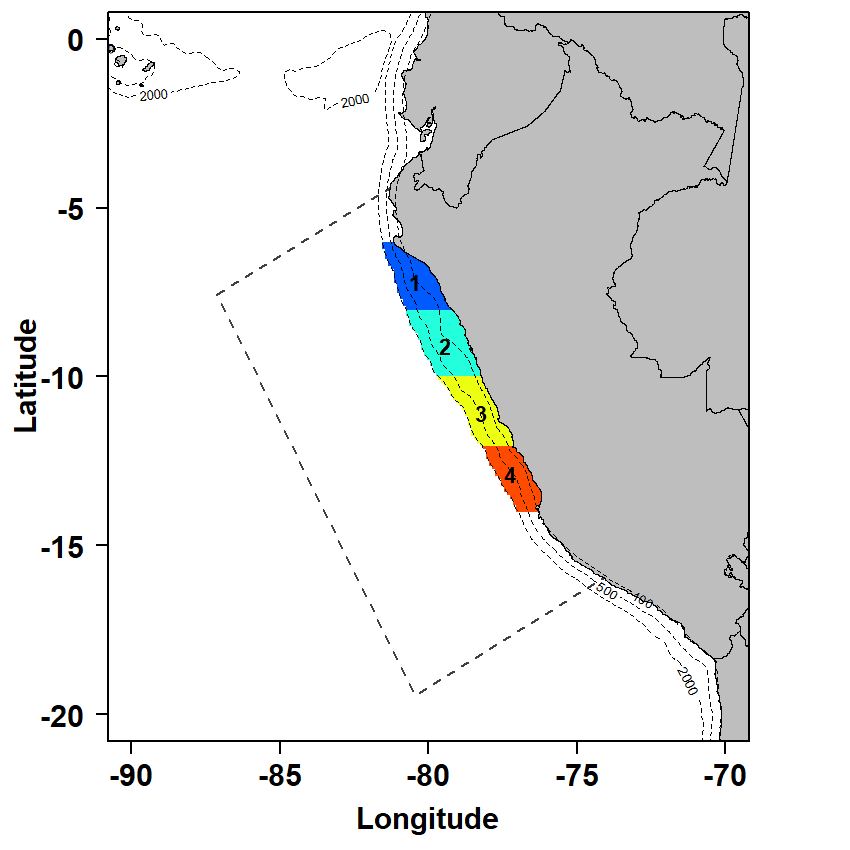
\includegraphics[width=1.0\textwidth]{figures/Chap2SpawningZone.png}
	\centering
	\caption{Domain of \acrshort{ibm} model study area at 10 km of spatial resolution ($D01$). Dotted rectangle represents the nested model domains ($D02s$, $D02s$) at 2 km resolution used for spatial resolution test. Release areas ($1 - 4$) are every $2$ degrees (\textdegree) of latitude between $6$\textdegree – $14$\textdegree $S$. Three isobaths ($100 m$, $500 m$ and $2000 m$) are shown.}
	\label{Chap2SpawningZone}
\end{figure}

\begin{figure}[H]
	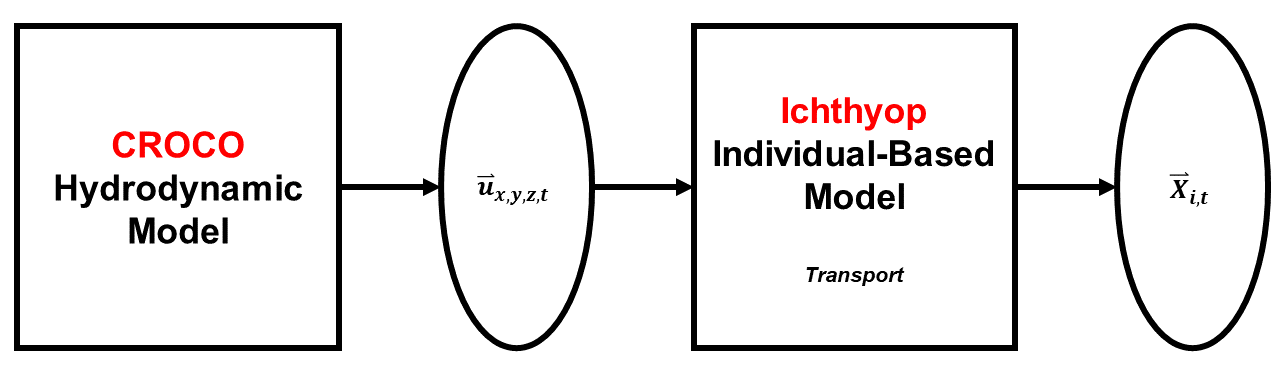
\includegraphics[width=1.0\textwidth]{figures/Chap2Ichthyop.png}
	\centering
	\caption{Representative flow diagram of the Ichthyop model and its hydrodynamic forcing using CROCO.}
	\label{Chap2Ichthyop}
\end{figure}

\subsection{Process overview and scheduling}\label{Chap2MethProc}

Virtual individuals were released in the physical environment according to a determined spatial (area, depth and bathymetry) and temporal (month and frequency) releasing strategy that constituted the initial conditions (section \ref{Chap2MethInit}). For each time step (2 hours), every egg or larva was transported by the 3D current fields. Finally, they were tested for recruitment on the continental shelf.\\

\subsection{Design concepts}\label{Chap2MethDesi}

\begin{itemize}

\item Stochasticity: Individuals were initially randomly distributed over the Peruvian continental shelf. We chose the number of individuals released ($5000$) such that the variability of simulated recruitment between three replicates of the same simulation was negligible.\\

\item Coastline behaviour: One of the utilities of \gls{ich} is the option to use different response configurations of a particle when faced with the decision of what to do when it touches the land boundary (coastline). We tested three types of coastline behaviours: 1) \textbf{BEACHING}: \gls{ich} does move the particle inland but ``kill'' it. From now onward the particle is out of the simulation. 2) \textbf{BOUNCING}: the coastline acts as a billard edge and the particle will bounce as a billard ball in the events that the move would take it beyond the coastline. The particle bounces back as much as it would penetrate inland and 3) \textbf{STANDSTILL}: the particle gives up on the move that would take it inland and just wait until next time step for trying another move.\\

\item Observation: After 30 days of drift, each particle was tested to see if it was within the continental shelf and was considered ``retained'' or ``non-retained''. From now on, we will call \gls{cri1}, referring ``retention'' as a criterion for larval recruitment.\\

\end{itemize}

\subsection{Initialization}\label{Chap2MethInit}

In each simulation, individuals were released randomly along the coastal release area each month at days $1$, $10$ and $20$, during the three climatological years used.\\

Release area (Fig. \ref{Chap2SpawningZone}) was defined between latitudes $6$\textdegree $S$ and $14$\textdegree $S$, depths $0 m$ to $45 m$ and from the coast to bathymetry contour $2000 m$. This area was further splitted into different subdomains for the simulations post-processing and analysis (released depth ranges $0-15 m$, $15-30 m$ and $30-45 m$; cross-shore extension delimited by isobaths $0-100 m$, $100-500 m$, $500-2000 m$).\\

\subsection{Sub-models}\label{Chap2MethSubMod}

\begin{itemize}

\item Transport: To simulate particle transport, virtual individuals were advected using a trilinear interpolation scheme of the velocity fields derived from \acrshort{croco}, in time and space, and using a forward Euler numerical scheme with horizontal diffusion following \cite{PeliMarc2007}.\\

\item Retention: We considered one age-criterion for recruitment, hereafter referred to as \gls{cri1}. An individual was considered as ``recruited'' if it was within the coastal zone (offshore limit: the $2000 m$ isobath) at age $30$ days.\\

\end{itemize}

\subsection{Simulations and sensitivity analysis}\label{Chap2MethSimSens}

From this chapter onwards, each drift simulation will be listed under the name ``\textbf{$sim \#$}'', for example, in the text, saying ``$sim 1$'', will be equivalent to saying ``\textit{simulation 1}''. Details of each simulation will be detailed in a table in its corresponding chapter.\\

Three simulations were performed in order to explore the model sensitivity to different environmental forcing fields (Table \ref{TabSimus}). In order to fit the spatial extent of the $2 km$ grid, individuals release was constrained in the coastal area between $6$\textdegree $S$ and $14$\textdegree $S$ (Fig. \ref{Chap2SpawningZone}, dotted box) for all three simulations. Larval recruitment was calculated at $30$ days (\gls{cri1}).\\

\clearpage
\section{Results}\label{Chap2Resu}

Simulated retention patterns obtained with the three tested configurations of the hydrodynamic model were very similar and did not show any significant differences on retention patterns related to the use of different spatial resolutions ($Sim 1$, $Sim 2$ and $Sim 3$, Fig. \ref{Chap2Recruitment3bars}). The main differences concerned the $D02s$ configuration ($Sim 2$) that exhibits slightly higher retention values for austral summer months (Fig. \ref{Chap2Recruitment3bars}a) and for the coastal spawning zone ($0-100m$ isobath, Fig. \ref{Chap2Recruitment3bars}d). The latitudinal range between $10$\textdegree - $12$\textdegree $S$ was the most favorable for larval retention (Fig. \ref{Chap2Recruitment3bars}b) and a direct relationship was observed between spawning depth and larval retention, being lower near the surface and higher in deeper layers (Fig. \ref{Chap2Recruitment3bars}c).\\

\begin{figure}[H]
	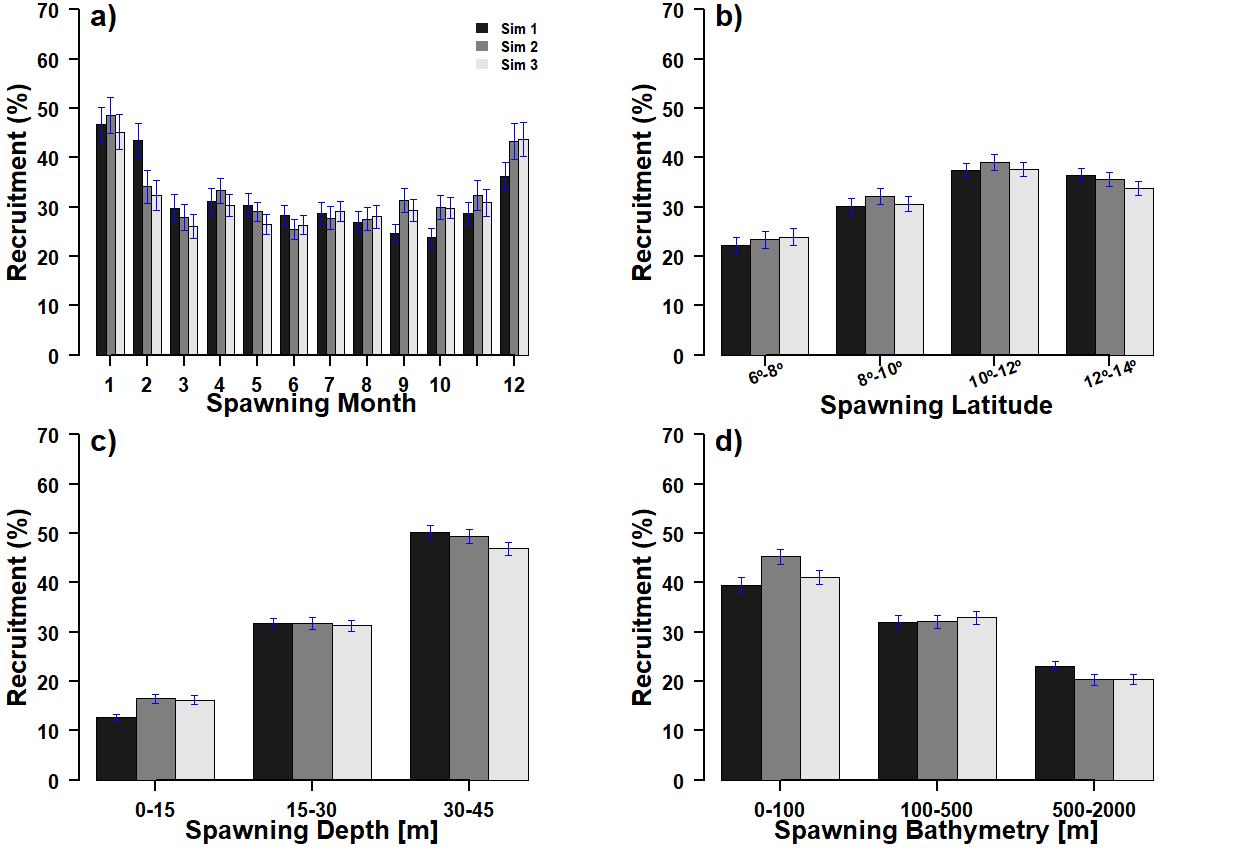
\includegraphics[width=1.0\textwidth]{figures/Chap2Recruitment3bars.png}
	\centering
	\caption{Percentage of recruited larvae of Peruvian anchovy using an age-criterion (\gls{cri1}) obtained for different (a) release months, (b) release latitudes, (c) release depths, and (d) isobaths delimiting releasing areas horizontally, for three simulations using forcing fields at different spatial resolution ($Sim 1$ in black, $Sim 2$ in dark grey, $Sim 3$ in light gray; see Table \ref{TabSimus} for details on simulations characteristics). Blue arrows represent confidence interval ($95 \%$).}
	\label{Chap2Recruitment3bars}
\end{figure}

An ANOVA (Table \ref{TabAnovaSimus}) was applied to evaluate which of the factors (release year, release month, release depth, release bathymetry, release latitude, horizontal resolution and coastline behaviour) and its interactions had the greatest impact. Release depth explained $28.32 \%$ of the variance and showed a direct relationship between release depth and retention rate, with higher values when the particles were released deeper ($30 - 45 m$) and lower values when they were released near the surface ($0 - 15 m$, $15 - 30 m$) (Fig. \ref{Chap2Recruitment3bars}c). Release bathymetry explained $12.27 \%$ of the variance, with the highest retention rates in the area closest to the coast ($0 - 100 m$) than those released offshore ($100 - 500 m$, $500 - 2000 m$) (Fig. \ref{Chap2Recruitment3bars}d). Release month explained only $4.95 \%$ of the variance and showed seasonal variability with the summer months having the highest retention rate (Fig. \ref{Chap2Recruitment3bars}a). Release latitude explained $4.47 \%$ of the variance and the zone between $10 - 12$\textdegree $S$ was the major latitudinal retention zone (Fig. \ref{Chap2Recruitment3bars}b). Finally, with an almost negligible percentage of variance explanation, are spatial resolution ($0.1 \%$), coastline behaviour ($0.04 \%$) and release year ($0.01 \%$).\\

The depth of release had the most significant effect in all three simulations. It interacted with the month of release and explained $10.15 \%$ of the variance of larval retention, affecting the seasonal pattern (Fig. \ref{Chap2Recruitment3sim3depth}). Particles released near the surface ($0-15 m$, Fig. \ref{Chap2Recruitment3sim3depth} a, d, g) showed a seasonal pattern favoring retention in the winter months, while this pattern reverses as release depth increases ($15 - 30 m$, Fig. \ref{Chap2Recruitment3sim3depth} b, e, h; $30 - 45 m$, c, f, i).\\

%\begin{landscape}
\begin{table}[H]
\centering
\begin{adjustbox}{width=1.2\textwidth}
\small
\begin{tabular}{c|r|r|r|r|r|r}
\hline
 							     &
  \textbf{Df} 				     &
  \textbf{Sum Sq} 			     &
  \textbf{Mean Sq} 			     &
  \textbf{F-value} 			     &
  \textbf{Pr (\textgreater{F})} &
  $\mathbf{\% Exp}$     		 \\
\hline
Year                             & 2     & 2251.49    & 1125.74    & 8.6851     & 1.69E-04  & 0.01110  \\
Month                            & 11    & 1004447.79 & 91313.44   & 704.4800   & 0.00E+00  & 4.95256  \\
Depth                            & 2  & 5743872.69 & 2871936.34 & 22156.8905 & 0.00E+00  & 28.32089 \\
Bathymetry                       & 2  & 2489211.28 & 1244605.64 & 9602.0899  & 0.00E+00  & 12.27337 \\
Latitude                         & 3  & 907672.24  & 302557.41  & 2334.2201  & 0.00E+00  & 4.47539  \\
Horizontal resolution            & 2  & 20531.36   & 10265.68   & 79.1994    & 4.81E-35  & 0.10123  \\
Coastline behaviour              & 2  & 8143.23    & 4071.62    & 31.4124    & 2.34E-14  & 0.04015  \\
Year x Month                     & 22 & 31614.97   & 1437.04    & 11.0867    & 3.40E-39  & 0.15588  \\
Year x Depth                     & 4  & 2620.20    & 655.05     & 5.0537     & 4.54E-04  & 0.01292  \\
Year x Bathymetry                & 4  & 4863.98    & 1215.99    & 9.3814     & 1.42E-07  & 0.02398  \\
Year x Latitude                  & 6  & 33678.38   & 5613.06    & 43.3046    & 5.20E-53  & 0.16606  \\
Year x Horizontal                & 4  & 4427.80    & 1106.95    & 8.5401     & 6.96E-07  & 0.02183  \\
Year x Coastline behaviour       & 4  & 7.67       & 1.92       & 0.0148     & 1.00E+00  & 0.00004  \\
Month x Depth                    & 22 & 2059893.93 & 93631.54   & 722.3641   & 0.00E+00  & 10.15657 \\
Month x Bathymetry               & 22 & 314249.09  & 14284.05   & 110.2010   & 0.00E+00  & 1.54944  \\
Month x Latitude                 & 33 & 1725393.57 & 52284.65   & 403.3743   & 0.00E+00  & 8.50727  \\
Month x Horizontal resolution    & 22 & 57626.98   & 2619.41    & 20.2086    & 8.84E-80  & 0.28414  \\
Month x Coastline behaviour      & 22 & 1194.51    & 54.30      & 0.4189     & 9.92E-01  & 0.00589  \\
Depth x Bathymetry               & 4  & 116211.66  & 29052.91   & 224.1422   & 2.65E-190 & 0.57300  \\
Depth x Latitude                 & 6  & 351244.70  & 58540.78   & 451.6401   & 0.00E+00  & 1.73186  \\
Depth x Horizontal resolution    & 4  & 11612.93   & 2903.23    & 22.3983    & 1.70E-18  & 0.05726  \\
Depth x Coastline behaviour      & 4  & 1362.45    & 340.61     & 2.6278     & 3.27E-02  & 0.00672  \\
Bathymetry x Latitude            & 6  & 765921.68  & 127653.61  & 984.8433   & 0.00E+00  & 3.77647  \\
Bathymetry x Horizontal resolution & 4 & 53546.30 & 13386.57 & 103.2770 & 1.37E-87 & 0.26402 \\
Bathymetry x Coastline behaviour   & 4 & 11584.89   & 2896.22    & 22.3443    & 1.89E-18  & 0.05712  \\
Latitude x Horizontal resolution   & 6 & 49319.27   & 8219.88    & 63.4161    & 1.20E-78  & 0.24317  \\
Latitude x Coastline behaviour     & 6 & 3020.05    & 503.34     & 3.8833     & 7.04E-04  & 0.01489  \\
Horizontal resolution x Coastline   behaviour & 4 & 1122.71  & 280.68   & 2.1654   & 7.02E-02 & 0.00554 \\
Residuals                        & 34754 & 4504751.04 & 129.62     &        &           & 22.21124\\
\hline
\end{tabular}
\end{adjustbox}
\caption{ANOVA of retention rates for $sim 1$ ($D01$), $sim 2$ ($D02s$) and $sim 3$ ($D02r$) combined.}
\label{TabAnovaSimus}
\end{table}
%\end{landscape}

Fig. \ref{Chap2SpatialVariation} showed that retention rates between $10$\textdegree $S$ - $12$ remained constant throughout the year in the 3 simulations, and interacting with release month, explained $8.5\%$ of the variance in retention. The northern zone between $6$\textdegree $S$ - $10$\textdegree $S$ showed seasonal variability with higher retention values in summer and accented values in January and February in $sim 2$ ($D02s$).\\

\begin{center}
\begin{figure}[H]
	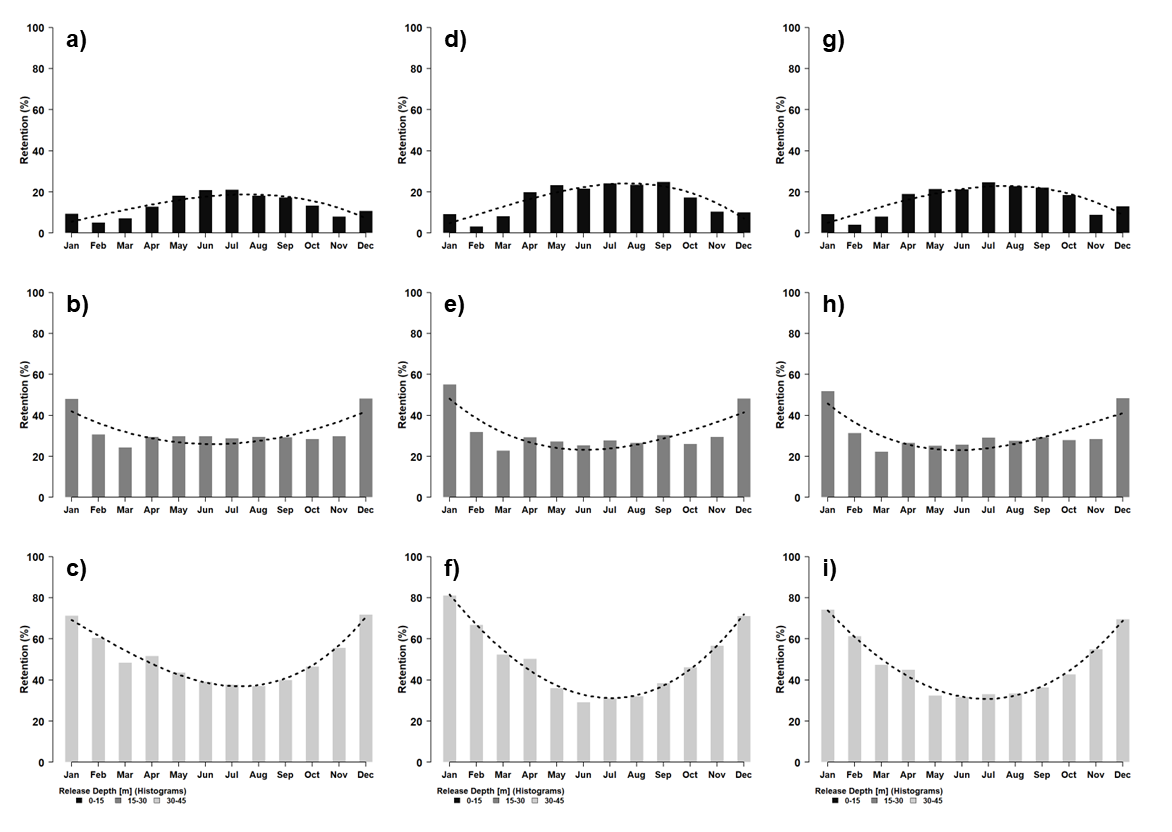
\includegraphics[width=1.0\textwidth]{figures/Chap2Recruitment3sim3depth.png}
	\centering
	\caption{Particle retention rates off Peru using 3 different physical forcing configurations ($D01$, a,b,c; $D02s$, d,e,f; $D02r$, g,h,i) and three release depths ($0 – 15 m$, $15 - 30 m$ and $30 - 45 m$).}
	\label{Chap2Recruitment3sim3depth}
\end{figure}
\end{center}

The remaining interactions among factors have a negligible effect, explaining less than $1\%$ of the variance in larval retention.\\

\begin{center}
\begin{figure}[H]
	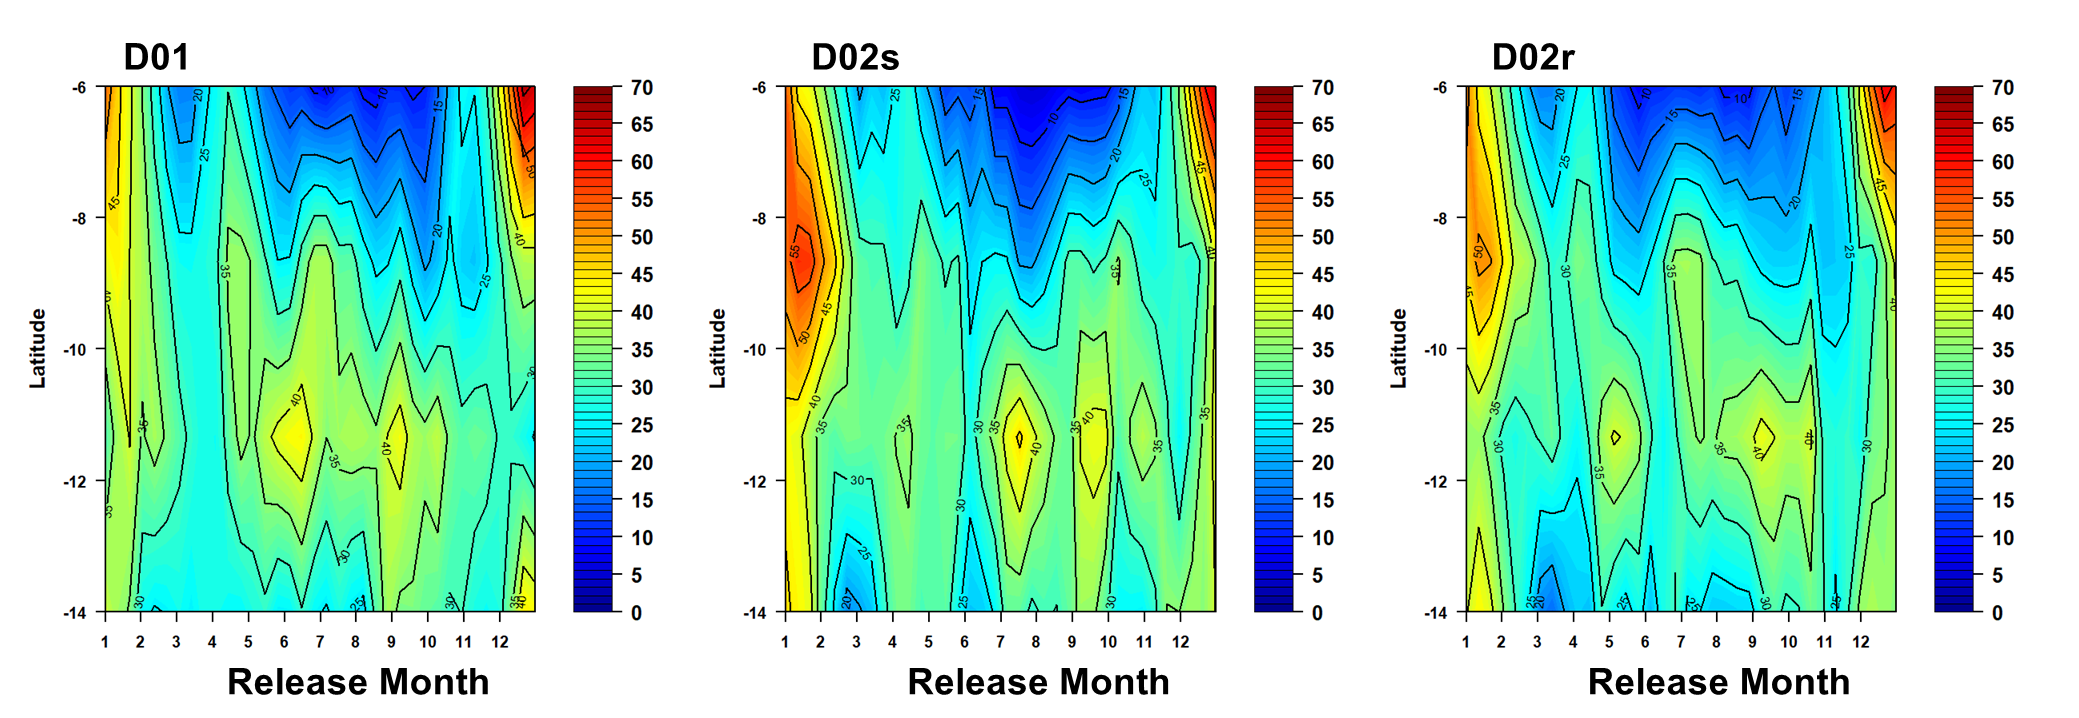
\includegraphics[width=1.0\textwidth]{figures/Chap2SpatialVariation.png}
	\centering
	\caption{Spatial variation of retention rates for $sim 1$ ($D01$), $sim 2$ ($D02s$) and $sim 3$ ($D02r$).}
	\label{Chap2SpatialVariation}
\end{figure}
\end{center}

\clearpage
\section{Discussion}\label{Chap2Disc}

A sensitivity analysis to spatial resolution and coastline behaviour was applied to the retention rates off Peru using \gls{ich} model, a powerfull Lagrangian tool \citep{LettVerl2008}. This tool allowed us to track virtual particles in a 3D environment and to know the location of each particle at each time step.\\

The fact that there was no significant difference between $sim 1$ ($D01$), $sim 2$ ($D02s$) and $sim 3$ ($D02r$) strengthen the conclusions found by \citep{BrocLett2008} who used a spatial resolution forcing only slightly greater than $10 km$, despite their study had a wider latitudinal range ($2$\textdegree - $20$\textdegree $S$) than the one used in this chapter ($6$\textdegree - $14$\textdegree $S$). \cite{BrocLett2008} also found that release depth is the most important factor ($22.7 \%$ of explained variance) although in a smaller proportion than in the present chapter ($28.32 \%$). However, \cite{BrocLett2008} found that the next most important factors were release latitude ($7.2 \%$) and then release bathymetry ($3.9 \%$), in contrast to the present chapter in which release latitude ($4.47 \%$) was less important than release bathymetry ($12.27 \%$). Concerning the release bathymetry, finding a higher value of percentage of variance explanation in this chapter compared to \cite{BrocLett2008}, could be due to the topographic sources \citep{SmitSand1997} used by them and the one used in the present chapter \citep{BeckSand2009} to represent the bathymetry, which could provide a better description of the seafloor and affect circulation and retention structures also affecting retention rates as \cite{RojaLand2014} reported.\\

\cite{LettPenv2007} applied Lagrangian simulation experiments to evaluate the processes of enrichment, retention and concentration proposed as the mechanisms that favor the recruitment of marine species \citep{Baku1998, Baku2010}. \cite{LettPenv2007} showed that after $20$ days of drifting, the zones of highest retention were located between grade $10$\textdegree $S$ - $14$\textdegree $S$, similar to our results in the $3$ simulations, values that were constant throughout the year in this latitudinal range, even though retention was calculated after $30$ days of drift. \cite{LettPenv2007} also showed a general seasonal pattern with the summer months favoring retention as well as in this chapter, however, we can now know that retention is highly dependent on initial depth (release depth), in agreement with \cite{BrocLett2008}, therefore, the larval retention of any species will depend on its spawning depth or its vertical behaviour \citep{OspiPara2012}.\\

A spatial resolution analysis was applied in the Humboldt ecosystem for one mollusk species \citep{GaraKapl2014}. Between $3 km$ and $7.5 km$ hydrodynamic forcings, no difference in dispersion distance was observed, however, both experiments also demonstrated that the closer to coast, the greater the success of the individuals, in this case called larval settlement (and retention in this chapter). It should be noted that they used much longer drift times ($80$ days and $140$ days).\\

The work did not evaluate the effect of wind forcing frequency (monthly winds and daily winds) at high resolution ($2 km$, $D02$) on retention rates while maintaining patterns, although this was applied only in very coastal and small areas at the scale of a bay \citep{FlorTam2019}.\\

This could have implications when we use different coastline behaviours, as demonstrated in this chapter, in which only beaching behaviour in areas very close to the coast ($0 - 100 m$) had significant impacts on retention rates, although did not have a major impact at level of the continental shelf off Peru, could have a significant effect if we study problems such as oil spills or accumulation of microplastics on the coast \citep{AtwoFalc2019,LopeNajj2021}.\\

Finally, we conclude that to work on \textit{\gls{ringens}} recruitment simulations, in order to save computational time and energy, we can continue with a spatial resolution of 10 km. In addition, it is recommended to use the coastal behaviour called standstill, since for the purposes of our research it will not significantly affect near-shore particle transport.\\
